\section{Architecture}
This section describes the internal architecture of Spring XD. The core of
Spring XD consists of modules. A \emph{module}\cite{modules} is a data processing
unit used by \emph{streams} and \emph{jobs}. Each module type is used to integrate with a specific
technology, such as HTTP or HDFS. Modules are bound together at runtime
to form a stream or job. Data is transferred between modules via a pluggable
messaging system. Spring XD \emph{container} (JVM) processes host module instances.
A typical Spring XD system will consist of multiple containers. A Spring XD
\emph{admin} (JVM) process is responsible for deploying modules to containers.
Apache ZooKeeper\cite{zookeeper} is used by admin and container processes
for overall coordination and process health monitoring. 
(See figure~\ref{fig:architecture}.)

\subsection{Application Context}
The foundation of Spring XD is the Spring \emph{application context}. The application
context is a dependency injection framework that is used to instantiate
objects along with their dependencies \cite{spring-framework-reference}.
The application context provides a consistent means of declaring dependencies
and configuration for applications written in Java. All projects in the
Spring\cite{spring} portfolio depend on the application context.

\subsection{Modules}
A Spring XD Module is a unit of data processing. A stream processing module
for Spring XD consists of one of three types: \emph{source}, \emph{processor}, and \emph{sink}.
A stream consists of a collection of modules that define a pipeline for data.
\emph{Job} modules are responsible for the execution of batch jobs. Modules are
covered in detail in section~\ref{sec:Modules}.

\subsection{Message Bus}
\label{subsec:MessageBus}
Modules require a data transport in order to transfer data. Spring XD
supports pluggable transports via a messaging abstraction known as 
the \emph{message bus}. Spring XD includes implementations based on Redis\cite{redis},
RabbitMQ\cite{rabbitmq}, and Kafka. Each of the message bus implementations are provided
by the Spring Integration project\cite{spring-integration-reference}.

\subsection{Containers}
A Spring XD container consists of a JVM running an application context which
loads child application contexts for modules on demand. Depending on the modules
being executed by the container, the container will also create connections to
the message bus. The container is responsible for reporting the status of its deployed
modules to the admin via ZooKeeper (see subsection~\ref{subsec:Admin}.)

Spring XD supports one or more containers within a cluster. The decision criteria
for selecting the number of containers is based on capacity requirements and/or access
to specific resources.  A typical Spring XD cluster has a base set of containers
running at all times so that streams or jobs can be created, deployed or launched
as needed. A user may spin up extra containers to handle the load during peak times
and then scale back as required.

A container may be associated with one or more groups. This functionality is useful
for targeting module deployments within a stream or job to specific containers.
For example, if a set of containers within a Spring XD cluster has access to
a Hadoop file system, that set of containers can be configured as the ``hdfs'' group.
This allows for streams that include the hdfs module to target deployment of
that module only to containers within the ``hdfs'' group.

\subsection{Admin}
\label{subsec:Admin}
The Spring XD admin server hosts a REST service used for Spring XD
administration and the orchestration of streams and jobs. While a single
admin server is required, multiple admin servers may be present in a Spring XD
system for redundancy. A single admin server will be responsible for stream
and job deployments. If multiple admin servers are present, a \emph{supervisor}
server will be selected via leadership election coordinated by ZooKeeper.
If more than one admin server is running, any of the admin servers
can service REST requests which helps load balancing the incoming requests.


\subsection{ZooKeeper}
Apache ZooKeeper is a distributed configuration and synchronization service.
It provides primitives required for the coordination of distributed systems.
In the case of Spring XD, ZooKeeper is used for: \begin{itemize*}
	\item Admin supervisor leadership election
	\item Centralized storage for stream and job definitions
	\item Centralized storage for runtime deployment properties
	\item Notification of stream/job deployments
	\item Tracking of containers and the modules they are hosting
	\item Notification of arriving and departing containers
\end{itemize*}
\begin{figure}[ht]
\centering
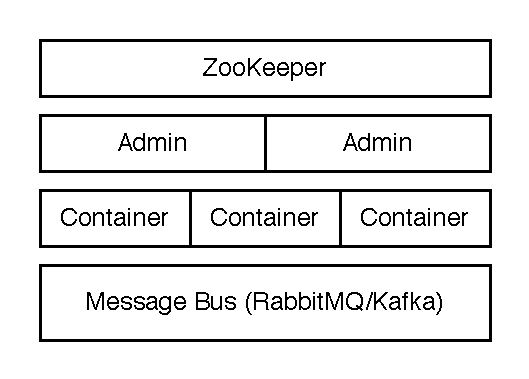
\epsfig{file=xd-architecture.eps, height=2in, width=3in}
\caption{Spring XD Architecture.}
\label{fig:architecture}
\end{figure}

